\part{Introduction}
\section{Foreword}
For the course 'kursusnavn' have it been required to conduct an investigation for a certain subject and then reflect over this subject. We have choosen to focus our attention on estimation techniques for development in software projects. Based on readings (kilde?) and own experience, we think that this subject have been a hard thing to do in and have often been a  troublesome task to perform. Because of this, we have chosen to base our investigation on estimates and more precisely estimation techniques given from the course book 'kilde'. 

\section{Background}
For this project we have to aim our investigation towards a certain project, to get some sensible data to analyse and reflect upon. We have chosen to use our second year project in the course 'Second Year Project: Software Development in Large Teams with International Collaboration'. In short, this project consists of a collaboration with a university group for a Singaporean university, where we been given the task to develop a server and a client for some kind of media service. The server will expose services which the Singaporean group will use to develop a client, which uses these services. We to, will have to make a client, which uses our servers services, but the collaboration and the serves services is the main objective of the project and there most of our attention will be. The project will start in February and go to the end of May, where the server and client code and a associated report of 20-30 pages will have to be handed in. \\ 

To help manage the project and reach our project deadline we will be using SCRUM (kilde til beskrivelse af scrum?) development method. This will enable us to apply different estimation techniques to the sprints, during the project period, which in the end will the techniques presented in this report. The team consists of 5 members with prior relationship to each other and with equal software developing experience in the required programming language. The project will be coded in the programming language C\#(kilde til C\# ?) and especially use .NET (kilde til .NET og WCF?)to expose the services on the server. It will be combined with a client developed in ASP.NET and HTML5. The later, is the only technology the team have not had any prior experience with and this will be a critical subject to investigate early in the project.  This leads to the overall complexity of the project, not being that great. The team consists of members, that all have experience with the required technologies except for HTML5, which being the only thing that requires in depth analysis, and the length of the project being fairly long.\\

Presented in the above, is a software project which will be conducted parallel to the writing of this report. The scope of the project is fairly proportioned to conduct the investigation. The project will give a good base for applying different estimations techniques and see how the works in a real project. 


\section{Problem definition}
For a software project, with the described size and scope, we will investigate and try certain estimation techniques and compares these. We will further discuss them and what other prerequisites that need to be obtained to successfully use the techniques and meet project deadlines. The questions below will outline the subjects that will be presented in the following report:  
\begin{itemize}
\item What prerequisites are necessary in order to perform accurate estimates of the workload in a software project?
\item How do different estimation techniques affect the teams' ability to meet project deadlines?
\item How does the working conditions influence the precision and usefulness of the various estimation techniques?	
\item Is one estimation technique more appropriate than others in a project of size and scope similar to a 4 month university project?
\newpage

\end{itemize}
\section{Motivation}
In the start of every software project, the first things that stakeholders, executive people and other similar persons are interested in, is the price of the project and the time frame that he project is about to enter. Questions like: "When can we expect the first prototype" and "When is the product ready to be shipped of to customers", are ones that often is needed to be answered in the start of a project typical by a manager. For the managers point of view, this can often be a challenge to answer, mainly due to the fact the 'requirements' for the project, at this point, are often vaguely defined and more a wish-list than actually requirements, that can be translated into program features. This combined with the fact, that developing a pierce of software from scratch often require a certain amount of innovation. Even though the project  will use known and common technologies and developing methods, these can be combined in a new way and this can both be time consuming and some time troublesome. \\
Because of this, many estimates for software project have been poorly and predicted delivery dates have often been exceeded with several percentages (KILDE OOA/D bogen). This could point towards that estimating projects should be handled by specialist which would have an objective view of the project, like its seen in civil engineering. Here an estimator does nothing else than trying to accurate estimate the tasks of the project. This means that estimates of civil engineering often are more precise than estimates in software projects. This is due to the fact, that in civil engineering when starting a project, its for the most time possible to use experience from earlier similar projects, which make the estimates more precise. \\
Clearly estimating in software projects is milestones behind civil engineering, where estimation specialist have a big importance among other things. Therefore a lot of research is done in the field of software engineering and many optimistic attempts have been made to develop estimating techniques, that tries to limit the chance of a estimations of tasks is so off, that it will impact the whole project and especially the final delivery date. 
Therefore we will, in the following sections, describe, discuss and analyse various estimating techniques and test some of them in a real software project. Many techniques have been developed and some have archived more success than others, but it is clear that we have to limit our scope and focus on only a couple of techniques. Because of this, the following sections will address the following techniques: Delphi, planning poker, PERT and .... . \\
We have choosen to limit our focus to these three, because of the prerequisites that is needed to use these techniques, among other things. Other techniques like 'CoComo' and 'function point analysis' requires things like experience from earlier similar projects, which the team does not have. The three techniques we will direct our attention towards, is not however the 'right' techniques or the ones that deliver the best results. These three techniques share the same chance of errors and fault with all other techniques. We have simply to focus on these, because we believe that this is the techniques that fits our project scope, size and complexity the best.\\
This concludes our thoughts about the background for choosing to focus on task estimation in a software project. The text above have outlined some important aspects about estimation for a software project and compared this with civil engineering. The main objective for the report will be to further describe and investigate some of the described things and in the end outline the major aspects for a certain estimations technique.

\section{Constraints}
Group size
Project size
Project duration
International cooperation
\section{Prerequisites}
As the focus of this project is to investigate and compare estimation techniques, it is paramount that the prerequisites for composing these estimates, such as understanding requirements, appropriately breaking down tasks etc, are considered thoroughly to minimize sources of error in our drawn conclusions. In this section, we will attempt to summarize the considerations made by the project group on this subject.

The course textbook makes the point that an estimate of the expected time consumption of a project, cannot be made without a clear understanding of the goal of the project. In a software development project, this largely equates to the requirements of the system under development. A comprehensive requirements analysis is somewhat out of of scope for this report, so the requirements artefacts which constitutes the product of the analysis efforts are deferred to the appendix, should the reader wish to review them.

In addition to the requirements analysis, the book emphasizes the importance of breaking down tasks into atomic units of work, that is units of work "that do not readily lend themselves to further subdivision or to assignment to more than one person", in order to accurately estimate their required duration. The authors proceed to suggest two approaches to breaking the project down to manageable, estimation friendly parts. The first proposed method, described as the more traditional of the two, is to break down the \textit{work} of the overall project into smaller units, and then break these down into smaller parts each, until a satisfactory level of granulation is reached. In the case of the media rental system it might look like this:

\begin{center}
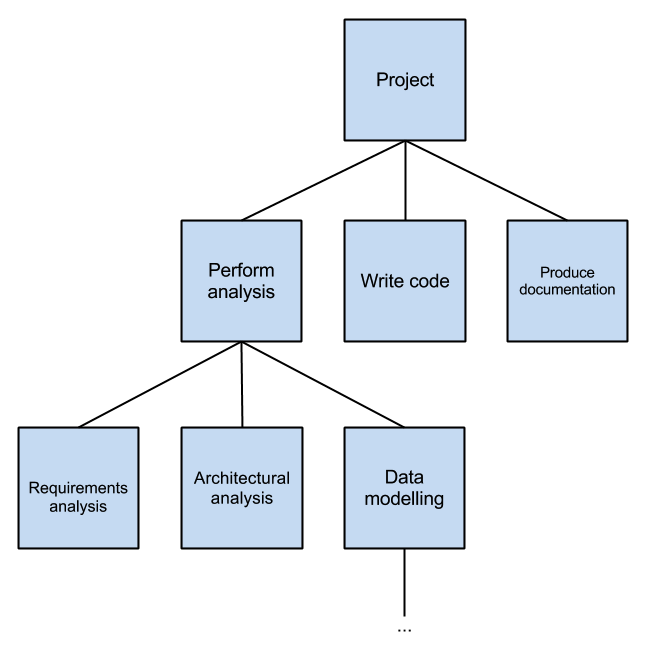
\includegraphics[scale=0.5]{TaskBreakdown.png}
\end{center}

In practice, the tasks would have to be broken down into finer subdivision in order to posses the quality of atomicity as defined in the literature.
